\documentclass[a4paper,12pt]{extarticle}
\usepackage{geometry}
\usepackage[T1]{fontenc}
\usepackage[utf8]{inputenc}
\usepackage[english,russian]{babel}
\usepackage{amsmath}
\usepackage{amsthm}
\usepackage{amssymb}
\usepackage{fancyhdr}
\usepackage{setspace}
\usepackage{graphicx}
\usepackage{colortbl}
\usepackage{tikz}
\usepackage{pgf}
\usepackage{subcaption}
\usepackage{listings}
\usepackage{indentfirst}
% \usepackage[
% backend=biber,
% style=numeric,
% maxbibnames=99
% ]{biblatex}

\usepackage[
  backend=biber,
  style=numeric,
  sorting=none,
  maxbibnames=99
]{biblatex}

\addbibresource{refs.bib}
\usepackage[colorlinks,citecolor=blue,linkcolor=blue,bookmarks=false,hypertexnames=true, urlcolor=blue]{hyperref} 
\usepackage{indentfirst}
\usepackage{mathtools}
\usepackage{booktabs}
\usepackage[flushleft]{threeparttable}
\usepackage{tablefootnote}

\usepackage{chngcntr} % нумерация графиков и таблиц по секциям
\counterwithin{table}{section}
\counterwithin{figure}{section}

\graphicspath{{graphics/}}%путь к рисункам

\makeatletter
% \renewcommand{\@biblabel}[1]{#1.} % Заменяем библиографию с квадратных скобок на точку:
\makeatother

\geometry{left=2.5cm}% левое поле
\geometry{right=1.0cm}% правое поле
\geometry{top=2.0cm}% верхнее поле
\geometry{bottom=2.0cm}% нижнее поле
\setlength{\parindent}{1.25cm}
\renewcommand{\baselinestretch}{1.5} % междустрочный интервал

\usepackage[hyphens]{url}

\newcommand{\bibref}[3]{\hyperlink{#1}{#2 (#3)}} % biblabel, authors, year
\addto\captionsrussian{\def\refname{Список литературы (или источников)}} 

\renewcommand{\theenumi}{\arabic{enumi}}% Меняем везде перечисления на цифра.цифра
\renewcommand{\labelenumi}{\arabic{enumi}}% Меняем везде перечисления на цифра.цифра
\renewcommand{\theenumii}{.\arabic{enumii}}% Меняем везде перечисления на цифра.цифра
\renewcommand{\labelenumii}{\arabic{enumi}.\arabic{enumii}.}% Меняем везде перечисления на цифра.цифра
\renewcommand{\theenumiii}{.\arabic{enumiii}}% Меняем везде перечисления на цифра.цифра
\renewcommand{\labelenumiii}{\arabic{enumi}.\arabic{enumii}.\arabic{enumiii}.}% Меняем везде перечисления на цифра.цифра


\counterwithout{figure}{section}

\begin{document}
\begin{titlepage}
\newpage

{\setstretch{1.0}
\begin{center}
ПРАВИТЕЛЬСТВО РОССИЙСКОЙ ФЕДЕРАЦИИ\\
ФГАОУ ВО НАЦИОНАЛЬНЫЙ ИССЛЕДОВАТЕЛЬСКИЙ УНИВЕРСИТЕТ\\
«ВЫСШАЯ ШКОЛА ЭКОНОМИКИ»
\\
\bigskip
Факультет компьютерных наук\\
Образовательная программа «Прикладная математика и информатика»
\end{center}
}

\vspace{2em}
УДК 004.8 % УДК нужно указывать только для исследовательсвого проекта - удалите эту строку для программного проекта
\vspace{4em}

\begin{center}
%Выберите какой у вас проект
{\bf Отчет об исследовательском проекте на тему:}\\
%{\bf Отчет о командном исследовательском проекте на тему:}\\
%{\bf Отчет о программном проекте на тему:}\\
%{\bf Отчет о командном программном проекте на тему:}\\
{\bf Редактирование изображений диффузионными
моделями при контекстно нетипичных текстовых
запросах}\\
% строчка ниже нужна только при сдача плана КР, при финальной сдаче закомментируйте ее
(промежуточный, этап 1)
\end{center}

\vspace{2em}

{\bf Выполнил студент: \vspace{2mm}}

{\setstretch{1.1}
\begin{tabular}{l@{\hskip 1.5cm}l}
группы \#БПМИ234, 3 курса & Карачун Александр Павлович \\
\end{tabular}}

% Обычно у вас есть один научный руководитель, и это человек, с которым вы работаете над проектом. Иногда по формальным причинам у вас будет руководитель (штатный сотрудник Вышки) и соруководитель (тот, с кем вы работаете), — об этом вам сообщит учебный офис (в случае с ВКР) или ЦППРиП (в случае с курсовым проектом). Также, если кто-то дополнительно вам помогал, то его можно указать как консультанта. 

%ваш официальный научник (из ВШЭ)
\vspace{1em}
{\bf Принял руководитель проекта: \vspace{2mm}}

{\setstretch{1.1}
\begin{tabular}{l}
Аланов Айбек\\

Старший научный сотрудник\\
НИУ ВШЭ
\end{tabular}}

\vspace{\fill}

\begin{center}
Москва 2026
\end{center}

\end{titlepage}% это титульный лист - выберите подходящий вам из имеющихся в проекте вариантов (kr - курсовая работа у 3 курса, vkr - выпускная квалификационная работа у 4 курса)
\newpage
\setcounter{page}{2}

{
	\hypersetup{linkcolor=black}
	\tableofcontents
}

\newpage

\newpage
\section*{Аннотация}   % this is how to use russian
В работе исследуется возможность использования знаний больших авторегрессионных vision-language моделей (VLM) для улучшения семантической точности генерации и редактирования изображений диффузионными моделями. Рассматривается подход VLM guidance, основанный на оптимизации латентных переменных диффузионной модели по градиенту функции согласованности изображения и текстового описания, вычисляемой с помощью VLM. В отличие от существующих методов, где оптимизируется только начальный латентный вектор, предлагается расширить оптимизацию на промежуточные латенты процесса денойзинга, а также исследовать возможность управления непрерывными параметрами генерации, такими как коэффициент classifier-free guidance и эмбеддинги null-text inversion.

Целью работы является проверка гипотезы о том, что градиенты VLM могут эффективно направлять генерацию в сторону сложных и нетривиальных семантик, выходящих за пределы обучающего распределения модели. Экспериментальная часть предполагает сравнение предложенного метода с современными базовыми моделями и существующими алгоритмами guidance по метрикам CLIP Score и Alignment на наборах промптов различной сложности.

Ожидается, что предложенный подход позволит повысить показатели семантического соответствия изображения тексту по сравнению с базовыми моделями, а также улучшить генерацию сложных композиционных и количественных концептов.



\addcontentsline{toc}{section}{Аннотация}

\section*{Ключевые слова}
Диффузионные модели, guidance, autoregressive VLM, оптимизация латентов, VLM-guidance, сложные семантики, редактирование изображений, classifier-free guidance, null-text inversion
\pagebreak

\addcontentsline{toc}{section}{Ключевые слова}

\newpage
\section{Введение}
% \addcontentsline{toc}{section}{Введение}
Диффузионные модели за последние годы стали стандартом для генерации и редактирования изображений по текстовому описанию. Современные архитектуры способны синтезировать фотореалистичные сцены, точно передавать стиль, освещение и текстуры, а также поддерживать разнообразные режимы управления — от inpainting \cite{mao2025unifyedit} до image-to-image \cite{blackforestlabs2025fluxkontext} трансформаций. В типичных сценариях, когда текстовый запрос описывает распространённые объекты и привычные композиции, качество генерации оказывается очень высоким.

Однако у этих моделей есть принципиальное ограничение: многие промпты оказываются для них семантически сложными. Это особенно заметно в случаях, когда текст содержит нетипичные для обучающего распределения концепты или их сочетания, редкие геометрические конфигурации, а также количественные требования. Например, композиционные конструкции («медведь делает стойку на передних лапах в парке»), структурные деформации объектов («гриб в лесу со сломанной пополам ножкой») или количественные требования («перчатка с шестью пальцами»). В подобных случаях модель часто генерирует визуально правдоподобную, но семантически некорректную сцену: игнорирует часть условий, «исправляет» нетипичную деталь на более вероятную либо создаёт гибридную интерпретацию запроса. Такие описания и соответствующие примеры генераций приведены на \autoref{fig:weird_prompts}.

С практической точки зрения эта проблема актуальна. В задачах генерации плохое понимание моделью семантики промпта часто приводит к неправильной генерации. В задачах редактирования, помимо этой проблемы, возникают и другие, например понимание моделью относительного расположения объектов на изображении. Таким образом, повышение семантической точности является краеугольным условием надёжного применения диффузионных моделей как инструмента контролируемого текстом редактирования и генерации изображений.

Корень описанной проблемы заключается в том, что диффузионные модели аппроксимируют распределение обучающих данных. Даже при условной генерации по тексту они склонны стремиться к наиболее привычным визуальным конфигурациям. Когда запрос требует выхода за пределы выученного распределения, например необычных количеств, нетривиальных пространственных отношений или логически противоречивых комбинаций, модель зачастую оказывается неспособна корректно удовлетворить этим требованиям.

\newpage

\begin{figure}[ht]
\centering

\begin{minipage}[t]{0.3\textwidth}
\centering
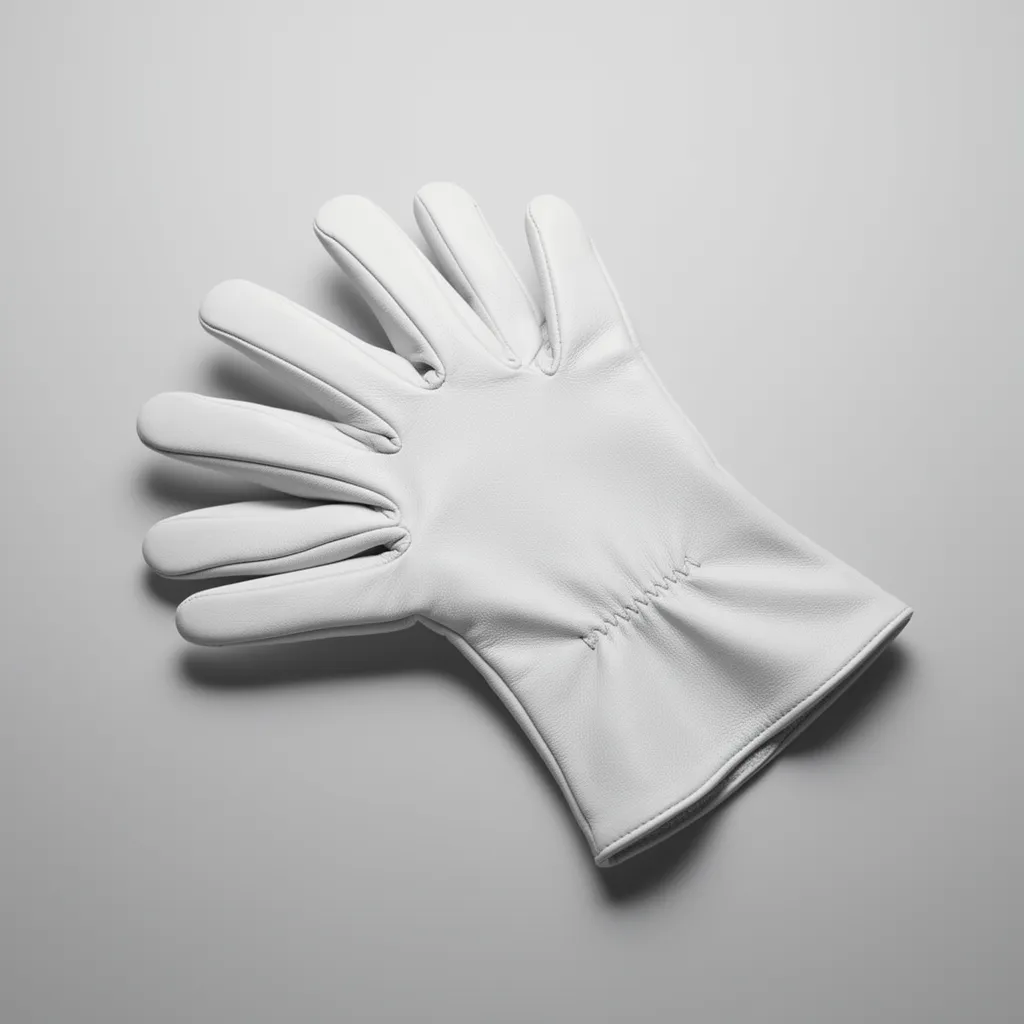
\includegraphics[width=\textwidth]{glove.png}

\small Промпт: «Белая перчатка с шестью пальцами»


\end{minipage}
\hfill
\begin{minipage}[t]{0.3\textwidth}
\centering
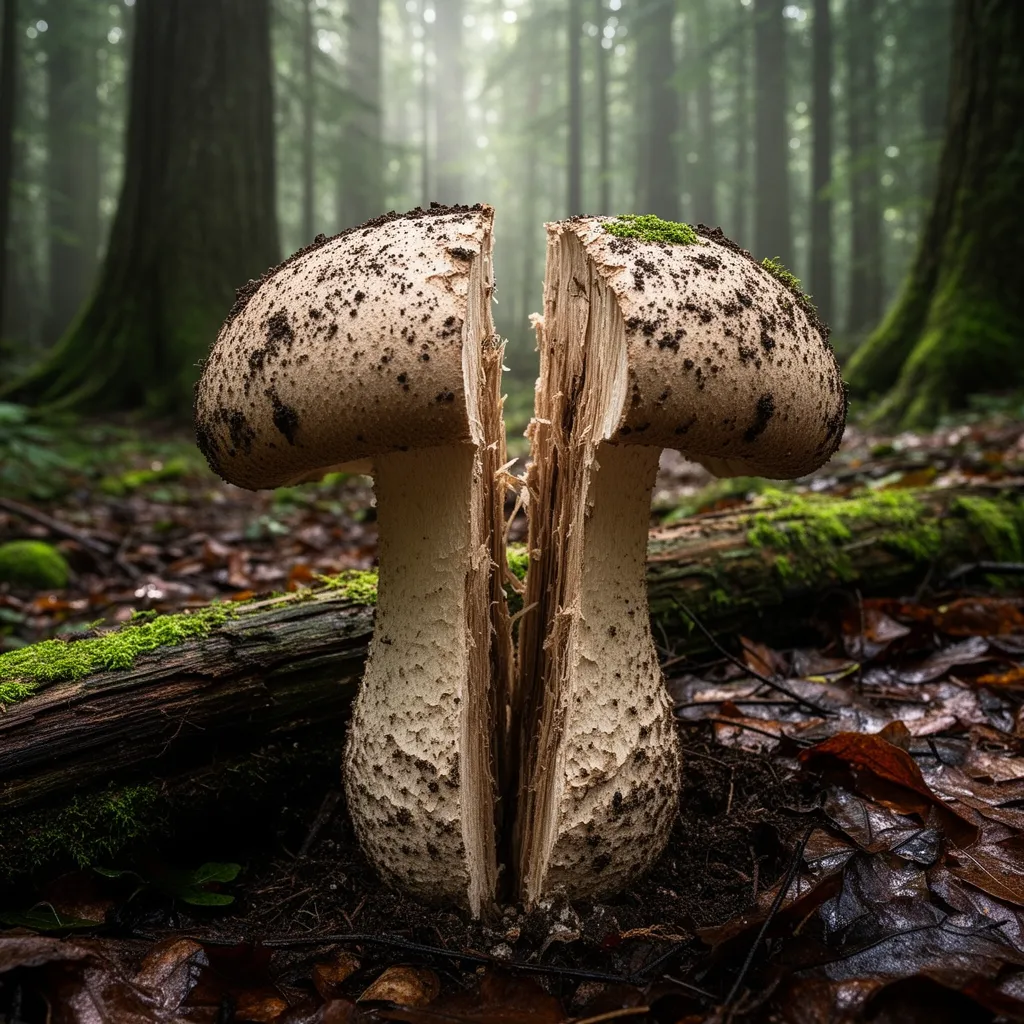
\includegraphics[width=\textwidth]{mushroom.png}

\small Промпт: «Гриб со сломанной пополам ножкой в лесу»


\end{minipage}
\hfill
\begin{minipage}[t]{0.3\textwidth}
\centering
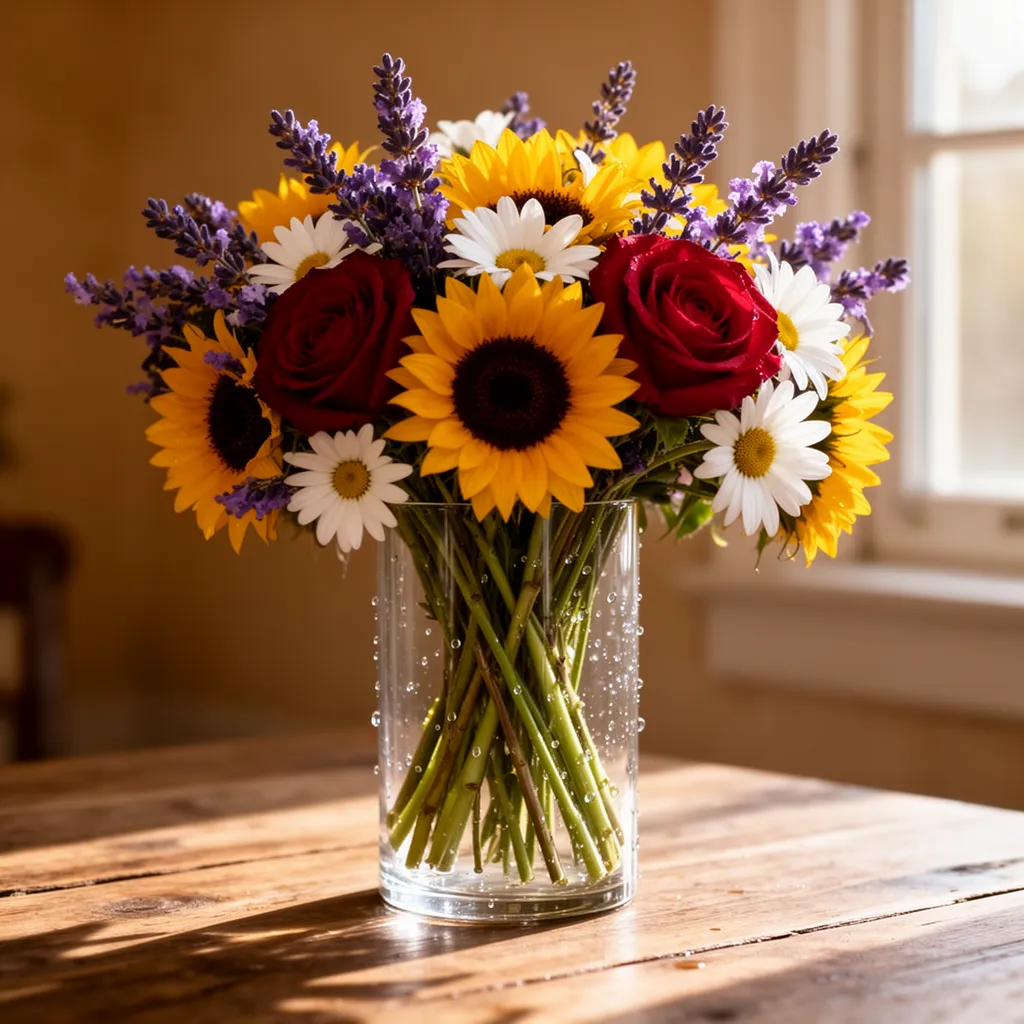
\includegraphics[width=\textwidth]{vase.png}

\small Промпт: «Букет цветов стоит в вазе вверх ногами»


\end{minipage}

\caption{Примеры генерации модели на семантически сложных промптах. Во всех случаях видно, как модель правдоподобно генерирует не соответствующие промпту изображения. Все генерации произведены по переведённым на английский язык промптам моделью FLUX.2[dev].}
\label{fig:weird_prompts}
\end{figure}

В то же время большие vision-language модели (VLM), обученные в авторегрессионной постановке, демонстрируют значительно более сильные способности к семантическому пониманию и проверке согласованности текста и изображения. Они способны понимать сложные языковые конструкции, учитывать контекст и выявлять несоответствия между визуальными и текстовыми данными. Это открывает возможность использовать VLM не только как инструмент оценки, но и как источник градиентного сигнала для управления процессом генерации.

Идея VLM guidance заключается в том, чтобы оптимизировать параметры генерации диффузионной модели по градиенту функции согласованности, вычисляемой VLM. В работе \cite{miao2024noisediffusion} было показано, что оптимизация стартового латентного представления может существенно повысить семантическую точность генерации сложных сцен. В данной работе эта идея развивается дальше: предлагается исследовать оптимизацию не только стартового латента, но и промежуточных латентных состояний в процессе денойзинга, а также других непрерывных параметров генерации. Такой подход потенциально позволяет воздействовать на семантику изображения не однократно в начале процесса, а последовательно корректировать её на протяжении всей траектории генерации.

Цель работы — экспериментально проверить гипотезу о том, что градиенты авторегрессионных VLM могут служить эффективным инструментом управления генерацией и редактированием изображений в случаях сложных, композиционных и количественных семантик. Для этого будет реализован пайплайн VLM-guided оптимизации и проведено сравнение с современными базовыми моделями по метрикам семантического соответствия (CLIP Score и alignment-оценкам на основе VLM) на наборах промптов различной сложности.

Ожидается, что предложенный подход позволит увеличить показатели семантической точности по сравнению с базовыми диффузионными моделями и, в частности, повысить устойчивость генерации в случаях, подобных приведённым на \autoref{fig:weird_prompts}. Кроме того, особое внимание будет уделено применимости метода к задаче редактирования изображений, где требования к сохранению исходного содержания и встраиванию в него корректировок делают проблему ещё более выраженной.

В дальнейшем работа организована следующим образом. В следующем разделе представлен обзор литературы по методам guidance и VLM-based управлению генерацией. Затем формулируется постановка задачи и описываются особенности рассматриваемых моделей и подходов guidance. После этого приводится описание предлагаемого пайплайна и экспериментального протокола. В заключении обсуждаются ограничения подхода и направления дальнейших исследований.



\section{Обзор литературы}

\paragraph{Диффузионные модели и механизмы guidance.}
Современные диффузионные модели являются стандартом для задач генерации изображений благодаря высокой фотореалистичности. Качество условной генерации в них во многом определяется механизмом \textit{guidance}~--- способом направленного изменения траектории обратного диффузионного процесса.

Ранние работы по \textit{classifier guidance} показали, что добавление градиента лог-вероятности класса к оценке шума позволяет управлять компромиссом между качеством и разнообразием генерации \cite{dhariwal2021diffusion}. Формально, если $\epsilon_\theta(x_t, t)$~--- оценка шума, а $\nabla_{x_t} \log p_\phi(y \mid x_t)$~--- градиент классификатора, то обновление принимает вид
\[
\tilde{\epsilon}_\theta = \epsilon_\theta + s \cdot \sigma_t \nabla_{x_t} \log p_\phi(y \mid x_t),
\]
где $s$~--- коэффициент guidance.

Позднее был предложен \textit{classifier-free guidance (CFG)}, позволяющий избежать обучения отдельного классификатора \cite{ho2022classifierfree}. В этом случае комбинируются условная и безусловная оценки шума:
\[
\epsilon_{\text{CFG}} = (1 + w) \epsilon_\theta(x_t, t, c) - w \epsilon_\theta(x_t, t, \emptyset)
\]
где $c$~--- текстовое условие, $\emptyset$~--- безусловный режим, $w$~--- коэффициент guidance.

Однако, несмотря на практическую эффективность, \textit{classifier-free guidance} в первую очередь усиливает уже присутствующую в модели условную компоненту, а не вводит новую семантическую информацию. По сути, коэффициент $w$ масштабирует разницу между условной и безусловной оценками шума, тем самым повышая выразительность признаков, коррелирующих с текстовым условием. Это приводит к улучшению семантической чёткости и согласованности с промптом, однако не гарантирует корректную реализацию сложных или редких композиционных структур. Если модель изначально не выучила определённую зависимость, например нетипичную пространственную конфигурацию или логически противоречивый атрибут, то увеличение $w$ лишь усиливает наиболее вероятные интерпретации, но не устраняет фундаментальные ограничения распределения. Таким образом, CFG частично решает задачу семантической точности за счёт усиления условного сигнала, но не обеспечивает полноценного контроля над сложными семантиками.

\paragraph{VLM-guidance и оптимизация латентов.}
Одним из направлений решения данной проблемы стало использование больших vision-language моделей (VLM) как более мощного семантического критерия. В работах по \textit{VLM-guidance} предлагается использовать функцию согласованности изображения и текста, вычисляемую через VLM, как сигнал для управления генерацией.

В частности, в работе Noise Diffusion вводится оценка $s(z_T)$, вычисляемая по изображению, полученному из начального шумового латента $z_T$ через процесс денойзинга, и вопросу о соответствии сэмпла промпту (VQA-score): $s(z_T)=\mathrm{VQA}(\cdot)$ \cite{miao2024noisediffusion}. Ключевая идея состоит в том, чтобы улучшать стартовый латент $z_T$, \emph{сохраняя распределение} $z_T \sim \mathcal{N}(0,I)$: вместо градиентного шага по $z_T$ применяется обновление, аналогичное прямому диффузионному процессу,
\[
z_T' = \sqrt{1-\gamma}\, z_T + \sqrt{\gamma}\, \sigma,
\qquad \sigma \sim \mathcal{N}(0,I),
\]
где $\gamma$~--- шаг (step size). В отличие от фиксированного шага, в работе $\gamma$ выбирается адаптивно в зависимости от текущего семантического качества:
\[
\gamma = 1 - \sqrt{s(z_T)}.
\]
Таким образом, при низком значении $s(z_T)$ шаг обновления становится более агрессивным, тогда как при высоком значении $s(z_T)$ обновление ослабляется.

Основная трудность --- подобрать шум $\sigma$, который увеличит семантическую оценку $s(\cdot)$. Для этого авторы в каждой итерации сэмплируют набор кандидатов $\{\sigma_i\}_{i=1}^N$, вычисляют соответствующие приращения
\[
v_i = z_T' - z_T
= (\sqrt{1-\gamma}-1)\,z_T + \sqrt{\gamma}\,\sigma_i,
\qquad i=1,\dots,N,
\]
и выбирают тот шум, для которого направление шага наиболее согласовано с оценкой градиента $\nabla_{z_T}s(z_T)$:
\[
\sigma^\star
= \arg\max_{\sigma_i}
\frac{\nabla_{z_T}s(z_T) v_i}{\lVert v_i\rVert_2^2}.
\]
После чего выполняется обновление
\[
z_T \leftarrow \sqrt{1-\gamma}\,z_T + \sqrt{\gamma}\,\sigma^\star,
\]
Такой шаг оптимизации происходит несколько раз итеративно.

\paragraph{VLM-gradient как обучающий сигнал для редактирования без пар.}
Отдельно важно направление, в котором VLM используется не только для inference-time guidance, но и как дифференцируемый сигнал при обучении модели редактирования без парных данных (оригинального и отредактированного изображения). В NP-Edit предлагается обучать диффузионную модель, опираясь на градиент VLM-оценки хода генерации отредактированной версии изображения \cite{kumari2025learning}.

\paragraph{Редактирование изображений и инверсия.}
В задачах редактирования дополнительным требованием является сохранение структуры исходного изображения, что во многом определяется точностью инверсии.

В работе Null-text Inversion показано, что оптимизация безусловного текстового эмбеддинга в рамках \textit{classifier-free guidance} позволяет значительно улучшить реконструкцию изображения и повысить устойчивость редактирования \cite{mokady2022nulltext}.

\paragraph{Stage-aware управление и proxy-prompts.}
Альтернативное направление представлено работами, в которых управление семантикой осуществляется не через градиенты, а через декомпозицию текстового условия по стадиям денойзинга. В частности, в подходе stage-aware prompt decomposition предлагается использовать последовательность proxy-prompts, адаптированных к различным фазам генерации \cite{huberman2025contextually}. Такой подход основан на наблюдении, что процесс диффузионной генерации носит \emph{coarse-to-fine} характер: на ранних шагах денойзинга формируется глобальная структура сцены и крупные композиционные элементы, тогда как на поздних шагах уточняются локальные детали, текстуры и мелкие атрибуты объектов.

Авторы показывают, что сложные или контекстно-противоречивые промпты могут перегружать модель на ранних этапах, когда необходимо прежде всего определить общую геометрию сцены. Поэтому предлагается сначала задавать более общие прокси-описания для формирования структуры, а затем постепенно уточнять семантику на более поздних шагах генерации. Такая стадийная декомпозиция позволяет частично повысить семантическую устойчивость и снизить вероятность противоречивых интерпретаций запроса.

Тем не менее данный подход воздействует на модель через изменение дискретного текстового условия и не обеспечивает прямого контроля над латентной траекторией. Кроме того, даже прокси-промпты могут оставаться семантически сложными для диффузионной модели, особенно в случаях количественных или нетипичных композиционных ограничений.

\paragraph{Позиционирование предлагаемого подхода.}
Существующие работы демонстрируют четыре ключевые идеи: (1) возможность управления диффузией через градиент внешней VLM-оценки верности семантики \cite{dhariwal2021diffusion,ho2022classifierfree}; (2) эффективность VLM как источника семантического сигнала \cite{miao2024noisediffusion,kumari2025learning}; (3) корень проблемы в воссоздании верной семантики именно ранних латентов \cite{huberman2025contextually}; (4) применимость оптимизации не только латентных непрерывных параметров для генерации \cite{mokady2022nulltext}.

В отличие от работ, где оптимизируется только начальный латент $z_0$, в данной работе предлагается исследовать оптимизацию промежуточных латентов $z_t$, а также непрерывных управляющих параметров (коэффициента CFG, null-text эмбеддингов и др.). Такой подход позволяет воздействовать на траекторию генерации на протяжении всего процесса денойзинга и потенциально обеспечивает более устойчивое выполнение сложных семантических ограничений как в задачах генерации, так и в задачах редактирования изображений.


\section{Планируемые результаты работы}

В результате выполнения работы будет разработан и выложен воспроизводимый экспериментальный пайплайн для VLM-guided генерации и редактирования изображений диффузионными моделями. Пайплайн будет включать реализацию оптимизации не только начального латента, но и промежуточных латентных состояний в процессе денойзинга, а также непрерывных управляющих параметров генерации (в частности, коэффициента classifier-free guidance и параметров, используемых в инверсии при редактировании, включая null-text эмбеддинги).

Будет реализован единый протокол экспериментов для text-to-image и image editing режимов, включающий подготовку наборов промптов различной сложности и стандартизированную процедуру генерации с фиксированным сидом, числом шагов денойзинга и бюджетом вычислений для сравнения методов.

Будет проведено количественное сравнение предложенного подхода с базовыми генераторами (SD1.5, SD3.0, FLUX.1[dev], FLUX.2[dev]) и с proxy-prompts подходом SAP \cite{huberman2025contextually}. Сравнение будет выполнено по метрикам семантического соответствия: CLIP Score (по протоколу из статьи Noise Diffusion \cite{miao2024noisediffusion}) и alignment на основе VLM (по протоколу из статьи SAP \cite{huberman2025contextually}) на наборах промптов разной сложности.

Будут получены отдельные результаты, характеризующие вклад каждого компонента предложенного подхода: оптимизации только $z_T$, оптимизации набора промежуточных $z_t$, совместной оптимизации $z_t$ и коэффициента CFG, а также (для редактирования) совместной оптимизации $z_t$ и null-text эмбеддингов. Для сравнения будет использован единый вычислительный бюджет, что позволит корректно сопоставить эффективность различных вариантов.

Будет подготовлен набор качественных результатов (визуальные примеры) для промптов с нетипичными композиционными и количественными ограничениями.

По итогам экспериментов будут сформулированы выводы о применимости VLM-gradient guidance для выхода за пределы prior диффузионных моделей в задачах генерации и редактирования, а также практические рекомендации по настройке пайплайна (какие латенты оптимизировать, на каких шагах, с каким шагом оптимизации и какие параметры управления дают наибольший эффект при заданном бюджете).




\newpage
\printbibliography[
  heading=bibintoc,
  sorting=none
]


\end{document}
